\section{Actuators and Sensors}

Below are attached the images that have been found regarding this. They are taken from the presentations given by \href{http://kiss.caltech.edu/workshops/smallsat2012b/presentations/mueller.pdf}{J.	Mueller} and \href{http://kiss.caltech.edu/workshops/smallsat2012b/presentations/bennett.pdf}{Matt Bennett}. 

\begin{center}
\begin{figure}[!ht]
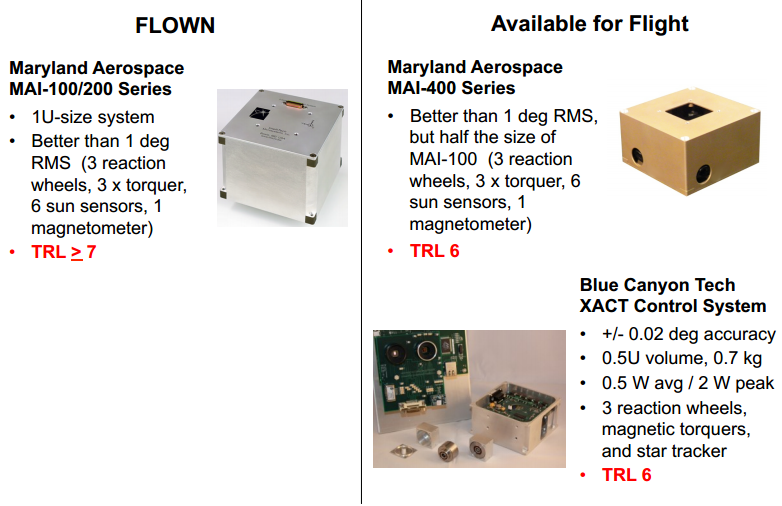
\includegraphics[scale=0.8]{attitude_control.png}
\caption{Current attitude control sensors and actuators}
\end{figure}
\newpage
\begin{figure}[!ht]
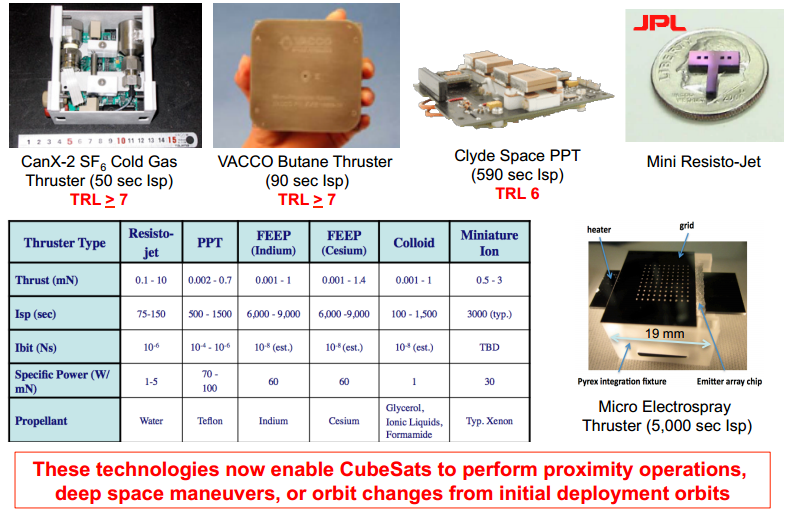
\includegraphics[scale=0.7]{prop_available.png}
\caption{Current thrusters}
\end{figure}
%\newpage
\end{center}
%\newpage

\begin{figure}[!ht]
\begin{center}
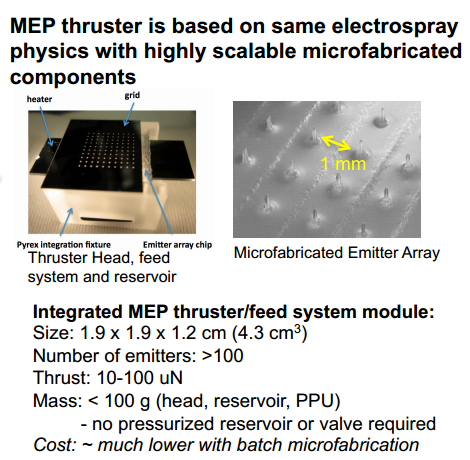
\includegraphics[scale=0.7]{MEP_prop.png}
\caption{Micro-Electric Propulsion specifications}
\end{center}
\end{figure}

This is not available of the shelf as of now. They had said it will take 1-2 years in December 2012. It will be a TRL 6 when it becomes available.  

Given below is a table showing what can be achieved using the state of the art controllers and actuators(as on December 2012). 

\begin{figure}[!ht]
\begin{center}
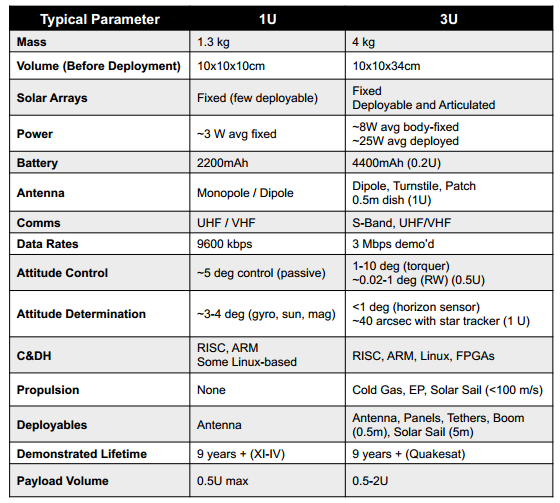
\includegraphics[scale=0.7]{state_of_art.png}
\caption{Current state of the art in all fields}
\end{center}
\end{figure}